\documentclass[a4paper,
fontsize=11pt,
%headings=small,
oneside,
numbers=noperiodatend,
parskip=half-,
bibliography=totoc,
final
]{scrartcl}

\usepackage{synttree}
\usepackage{graphicx}
\setkeys{Gin}{width=.4\textwidth} %default pics size

\graphicspath{{./plots/}}
\usepackage[ngerman]{babel}
\usepackage[T1]{fontenc}
%\usepackage{amsmath}
\usepackage[utf8x]{inputenc}
\usepackage [hyphens]{url}
\usepackage{booktabs} 
\usepackage[left=2.4cm,right=2.4cm,top=2.3cm,bottom=2cm,includeheadfoot]{geometry}
\usepackage{eurosym}
\usepackage{multirow}
\usepackage[ngerman]{varioref}
\setcapindent{1em}
\renewcommand{\labelitemi}{--}
\usepackage{paralist}
\usepackage{pdfpages}
\usepackage{lscape}
\usepackage{float}
\usepackage{acronym}
\usepackage{eurosym}
\usepackage[babel]{csquotes}
\usepackage{longtable,lscape}
\usepackage{mathpazo}
\usepackage[normalem]{ulem} %emphasize weiterhin kursiv
\usepackage[flushmargin,ragged]{footmisc} % left align footnote
\usepackage{ccicons} 
\setcapindent{0pt} % no indentation in captions

%%%% fancy LIBREAS URL color 
\usepackage{xcolor}
\definecolor{libreas}{RGB}{112,0,0}

\usepackage{listings}

\urlstyle{same}  % don't use monospace font for urls

\usepackage[fleqn]{amsmath}

%adjust fontsize for part

\usepackage{sectsty}
\partfont{\large}

%Das BibTeX-Zeichen mit \BibTeX setzen:
\def\symbol#1{\char #1\relax}
\def\bsl{{\tt\symbol{'134}}}
\def\BibTeX{{\rm B\kern-.05em{\sc i\kern-.025em b}\kern-.08em
    T\kern-.1667em\lower.7ex\hbox{E}\kern-.125emX}}

\usepackage{fancyhdr}
\fancyhf{}
\pagestyle{fancyplain}
\fancyhead[R]{\thepage}

% make sure bookmarks are created eventough sections are not numbered!
% uncommend if sections are numbered (bookmarks created by default)
\makeatletter
\renewcommand\@seccntformat[1]{}
\makeatother


\usepackage{hyperxmp}
\usepackage[colorlinks, linkcolor=black,citecolor=black, urlcolor=libreas,
breaklinks= true,bookmarks=true,bookmarksopen=true]{hyperref}
\usepackage{breakurl}

%meta
%meta

\fancyhead[L]{B. Kaden\\ %author
LIBREAS. Library Ideas, 35 (2019). % journal, issue, volume.
\href{http://nbn-resolving.de/}
{}} % urn 
% recommended use
%\href{http://nbn-resolving.de/}{\color{black}{urn:nbn:de...}}
\fancyhead[R]{\thepage} %page number
\fancyfoot[L] {\ccLogo \ccAttribution\ \href{https://creativecommons.org/licenses/by/4.0/}{\color{black}Creative Commons BY 4.0}}  %licence
\fancyfoot[R] {ISSN: 1860-7950}

\title{\LARGE{Ein Nachruf auf Professor Walther Umstätter}}% title
\subtitle{(* 12. Juni 1941 in Ploiești, Königreich Rumänien; † 6. März 2019 in Altlandsberg)}
\author{Ben Kaden} % author

\setcounter{page}{1}

\hypersetup{%
      pdftitle={Ein Nachruf auf Professor Walther Umstätter},
      pdfauthor={Ben Kaden},
      pdfcopyright={CC BY 4.0 International},
      pdfsubject={LIBREAS. Library Ideas, 35 (2019).},
      pdfkeywords={Nachruf, Walther Umstätter, obituary},
      pdflicenseurl={https://creativecommons.org/licenses/by/4.0/},
      pdfcontacturl={http://libreas.eu},
      baseurl={http://libreas.eu},
      pdflang={de},
      pdfmetalang={de}
     }



\date{}
\begin{document}

\maketitle
\thispagestyle{fancyplain} 

%abstracts

%body
\begin{figure}[h]
\centering
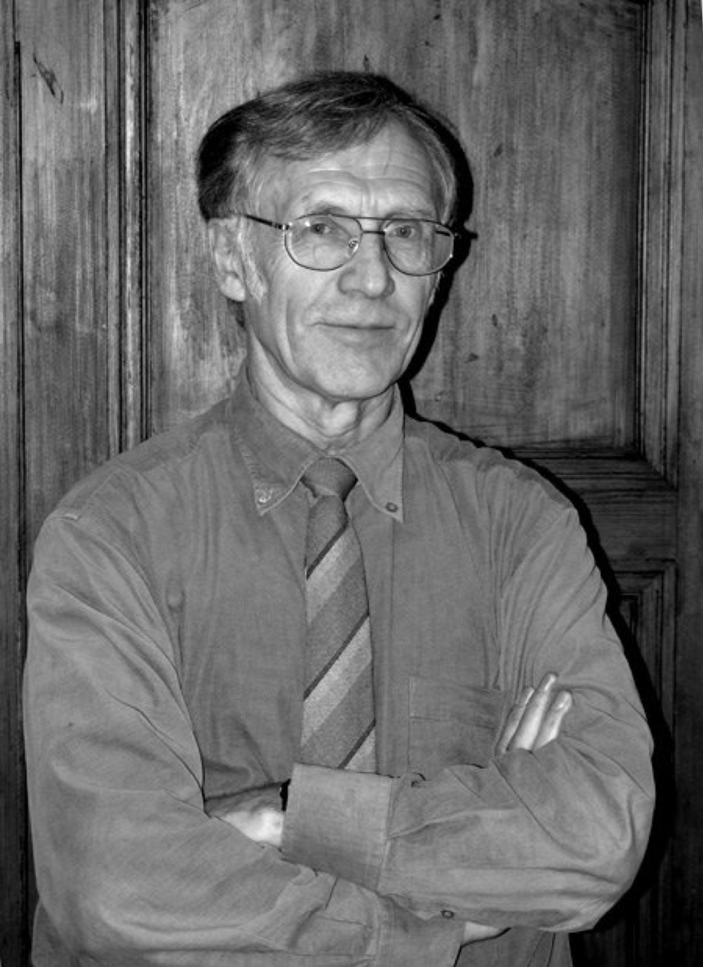
\includegraphics[width=.5\textwidth]{img/umstaetter.png}
\caption{Prof.~Dr.~Walter Umstätter}
\end{figure}

Es war eine einzige Frage, die entschied, ob mein Kommilitone Tuisko
oder ich die Stelle als studentischer Mitarbeiter am Lehrstuhl von
Professor Umstätter bekommen sollte. Wir waren drei oder vier Semester
am Institut, was für uns Magister-Studierende wenig bedeutete, denn wir
studierten ohnehin alles Mögliche, ziemlich ahnungslos, querbeet und
wenig davon an der Universität. In der Rückschau bereut man diese
Ziellosigkeit ein wenig, eigentlich sogar sehr, denn um die
Jahrtausendwende konnte die Humboldt-Universität mit einem unglaublichen
intellektuellen Potential aufwarten, einer ganz eigentümlichen
Ost-West-Mischung mit einem hohen Anteil an Akteuren, deren
Nebeneinander oft genauso zusammengewürfelt wirkte, wie es eben auch
war. Daraus resultierten Dissonanzen und zugleich viele Freiräume. Wie
die Stadt so die Universität, bemüht um Konsolidierung, darin jedoch,
als wäre sie ständig überfordert. Das Institut für
Bibliothekswissenschaft war dahingehend keine Ausnahme und unsere
eigenen Biografien alters- und naturgemäß zumindest in dieser Linie
sowieso im Takt. Eigentlich wollten fast alle, die man am Institut traf,
etwas Anderes machen. Auch ich wollte nie Bibliothekswissenschaft
studieren, aber in aller Ratlosigkeit nach einem abgebrochenen Semester
Amerikanistik im wintergrauen Potsdam-Golm und dem Zivildienst schien es
eine gemütliche Option im Immatrikulationsbüro Unter den Linden. Zur
Orientierung, bis sich herausstellt, was eigentlich werden soll. Das
erste Semester wurde, wie es sich traf, sowieso weitgehend verstreikt.

Im zweiten Semester gab es eine Vorlesung zur Einführung in die
Bibliothekswissenschaft bei Professor Umstätter, deren Gegenstand sehr
wenig mit Bibliotheken zu tun hatte und sehr viel mit einer überraschend
drastischen Dekonstruktion von Fachinformationsprogrammen und einem
einführenden Handbuch in die Grundlagen der praktischen Information und
Dokumentation. Als Einführungsvorlesung denkbar untauglich war es eine
beeindruckende methodische Schule, darin die Botschaft zirkelnd, dass
kritisches, zerlegendes Denken die Essenz von Wissenschaft sein kann.
Professor Umstätter erschien als Autorität, konzentriert auf die Sache,
deutlich weniger nahbar, zugleich deutlich weniger autoritär als Andere.
Er hatte ein Buch aktualisiert, aber eigentlich neu geschrieben,
gemeinsam mit Gisela Ewert. Das Lehrbuch der Bibliotheksverwaltung. Nach
dem zweiten Semester der bibliothekswissenschaftlichen Konfusion, als
einzig eine verpasste Frist den Fachwechsel verhindert hatte, ging ich
in den Semesterferien in ein kleine, längst nicht mehr existierende
Buchhandlung und bestellte es, über 60 Mark teuer, zur Verwunderung des
Händlers und auch zu meiner eigenen. Wenn schon noch ein Semester, dann
wollte ich es doch ernst nehmen. Ich las erst selektiv, dann
systematisch und mit dem Beginn des dritten Semesters wusste ich, was
man in Berlin unter Bibliothekswissenschaft verstehen konnte.

\begin{quote}
\enquote{Die Bibliothek ist eine Einrichtung, die unter archivarischen,
ökonomischen und synoptischen Gesichtspunkten publizierte Information
für die Benutzer sammelt, ordnet und verfügbar macht.}
\end{quote}

Auf dieser Definition konnte man aufbauen, verstehen und Ansätze finden.
Es gab nun also einen Grundstock, der sich als sehr hilfreich erwies,
wenn man einerseits die Breite, die das Studium selbst bot -- man
besuchte, heute unvorstellbar, erst ein Seminar zur Geschichte der
Kinderbuchillustration und danach eines zur gefühlt höheren Mathematik
-- irgendwie auf einen Bezugspunkt zusammenführen wollte und mehr noch
die Breite, die die Dynamik des fachlichen Ansatzes von Professor
Umstätter bot. Sputnik-Schock, Semiotik und Szientometrie, dazu
Kybernetik und die ewig kontroverse Frage nach der Unterscheidung
zwischen Daten, Information und Wissen. Die Situation an der
Humboldt-Universität ermöglichte ihm in der Lehre, seinen Herzensthemen
erstaunlich frei in einer höchst idiosynkratischen Mischung und nur mit
begrenzter Rücksicht auf die Verständnishorizonte und auch Interessen
zahlreicher Studierender zu entfalten. Seine Seminare waren eine
Herausforderung, doch wer durchhielt, nahm Bleibendes mit, was durchaus
positiv gemeint ist. Er verstand die grundsätzliche Bedeutung des
Digitalen für die Bibliotheken und für die Gesellschaft früher als die
Meisten, wusste das auch und verzweifelte nicht selten daran, wie wenig
seine Impulse, Vorschläge und Ideen aufgegriffen wurden. Derek de Solla
Price war ein Leitstern, Eugene Garfield ein anderer. Der eine, weil er
Wissenschaft als System durchschaubar und quasi berechenbar gemacht
hatte, der andere, weil er es verstand, aus diesem Wissen ein
wissenschaftsgestaltendes Geschäftsmodell zu generieren.

Eine Community fand er eher in der Gesellschaft für
Wissenschaftsforschung als im Bibliothekswesen, was ihn, wie für dieses
Fach fast traditionell prägend, zwischen den Stühlen platzierte.
Durchaus weithin geschätzt fand er sich in der Forschung sehr oft in
Zusammenhängen, die ihm weniger Raum ließen für das, was ihm wichtig
war. Ursprünglich kam er aus der Biologie mit dem Schwerpunkt
Pflanzenphysiologie und hin und wieder schlug sich das in der Frage
\enquote{Haben Pflanzen Wissen?} nieder, mit der er Studierende zum
Nachdenken motivieren wollte, denen allerdings häufig zahlreiche
Zwischenschritte und bisweilen auch das Interesse fehlte, um zu
verstehen, worin diese Frage wurzelte und warum sie sich mit der
\enquote{biogenetischen Evolutionsstrategie} befassen sollten, wo es
eigentlich um Fragen der Dokumentation ging. Der von ihm intensiv
gepflegte Rekurs auf die Informationstheorie von Claude Shannon und
Warren Weaver hätte mehr Entgegenkommen benötigt, um akzeptiert zu
werden.

Während die lange Zeit als Zukunftskonzept verhandelte Dokumentation
sonderbarerweise als Konzept verblasste, gewann die Bibliometrie seit
den 1990ern auch im Bibliothekswesen an Bedeutung, aber wenn, dann als
möglichst leicht anwendbares Werkzeug der Wissenschaftsmessung. Auch das
also keine Basis für eine wissenschaftliche Profilbildung mit größerem
Echo. Insgesamt blieb sie im Schatten anderer Trendthemen vorwiegend
betriebswirtschaftlicher Art und die Bibliothekspraxis forderte von der
Bibliothekswissenschaft entsprechende Lösungen. Gleichzeitig war das
Fach zu klein und darin zusätzlich zu disparat, blieb das
Bibliothekswesen zu sehr an konkreten Lösungen und zu wenig an Theorie
interessiert, um Professor Umstätter tatsächlich die wissenschaftliche
Entfaltungsfläche zu bieten, die er spürbar suchte und eigentlich auch
verdient hätte. Ab 2002 ging es in der Dorotheenstraße ohnehin fast nur
noch darum, die Löschung des Fachs aus der deutschen
Wissenschaftslandschaft zu verhindern. Die eigentliche Forschung wurde
zum Nebenschauplatz.

Aber auch unabhängig davon blieb oft der Eindruck, ihm fehlten
Gesprächspartner*innen, mit denen er seine Ideen und Theorien wirklich
diskutieren, spiegeln, aktualisieren und verfeinern konnte. Sie klangen
nicht selten zunächst irritierend, waren jedoch an vielen Stellen
erstaunlich ihrer Zeit voraus, hier und da vielleicht eher noch neben
ihr.

Obwohl er vermutlich der einzige Professor am Institut während der
1990er und 2000er Jahre war, der tatsächlich eine Generation von
Nachwuchswissenschaftler*innen wirklich wissenschaftlich prägen und
damit eine Art bibliothekswissenschaftliche Schule hätte begründen
können, gelang dies nur indirekt und in sehr kleinem Umfang. Er bemühte
sich beeindruckend, ausdauernd und unglaublich unterstützend um die bei
ihm Promovierenden. Wo er spürte, dass jemand für ein Thema, für die
Wissenschaft als Wissenschaft brannte, gab er alle Unterstützung, auch
wenn als Ergebnis etwas stand, was nicht auf seiner Linie lag. Er setzte
Impulse sowohl thematischer als auch methodischer und methodologischer
Art gerade dort, wo man sich von ihm abzugrenzen versuchte. Leider war
die Bibliothekswissenschaft keine Disziplin für wissenschaftliche
Karrieren und auch wenn unter den von ihm betreuten Promotionen und
Abschlussarbeiten eine Reihe exzellenter, genuin
bibliothekswissenschaftlicher Studien waren, eröffnete sich kaum
jemandem unter diesen Autor*innen eine Perspektive in der
bibliothekswissenschaftlichen Forschung.

Ich vermag nicht zu sagen, ob er das bedauerte und ich bin mir auch gar
nicht sicher, ob er meine Einschätzungen teilen würde. Ich durfte ihn
ein paar Jahre begleiten, in denen sich sehr viel am Institut und
naturgemäß auch für mich persönlich verschob und veränderte. Ich habe
eine differenzierte Position zur Informationstheorie entwickelt und mich
viel Semiotik befasst. Ideen der Dokumentation und der Anspruch von
Synopse und Vermittlung sind zentral in meinen Überlegungen zum Phänomen
der Bibliotheken. Wir waren uns in Vielem, auch Grundsätzlichem uneins,
aber er hat meinen Blick auf die Wissenschaft und die Auswahl der
Themen, mit denen ich mich befasste und immer noch befasse, maßgeblich
beeinflusst. Was ich also sicher sagen kann, ist, dass er zumindest
mich, aber vermutlich tatsächlich alle, die bei ihm lernten, so oder so
prägte und dass alle, die durchhielten und sich bei ihm mit einer Arbeit
qualifizierten, sehr viel von ihm mitnehmen und verinnerlichen konnten.
Man trifft in der Regel nicht allzu viele Menschen im Leben, die solche
Spuren hinterlassen. Und für jede dieser Begegnungen sollte man zutiefst
dankbar sein. Ich bin Professor Umstätter sehr dankbar, angefangen bei
der Einladung zum Vorstellungsgespräch für die Stelle eines
studentischen Mitarbeiters. Seine Frage war: Können Sie sich vorstellen,
auch nach Ihrem Studium in der Bibliothekswissenschaft zu bleiben? Ich
blieb und vermutlich nur aus diesem Grund.

(Berlin, 17.04.2019)

%autor
\begin{center}\rule{0.5\linewidth}{\linethickness}\end{center}

\textbf{Ben Kaden} ist Bibliothekswissenschaftler und Mitherausgeber von
LIBREAS. Er war von 2001 bis 2006 studentischer Mitarbeiter bei
Professor Walther Umstätter.

\end{document}
